\documentclass[addpoints,12pt]{exam}
%\usepackage[fontsize=18pt]{scrextend}
\newcommand{\ds}{\displaystyle}
\usepackage[margin=0.8in]{geometry}
\usepackage{subcaption}
\usepackage{pgfplots}
\usepackage{multicol}
\pgfplotsset{compat=1.16}

\usepackage{amssymb,amsmath,graphicx,wrapfig,verbatim, psfragx,color,todonotes}
\usepackage{multicol}
\usepackage{wasysym}
\newcommand*{\Scale}[2][4]{\scalebox{#1}{\ensuremath{#2}}}%

% \usepackage{amssymb,amsmath,graphicx,wrapfig,verbatim, psfragx,color}
% \usepackage{multicol}
% \usepackage{wasysym}
\usepackage{tikz}
\usetikzlibrary{fit}
\usetikzlibrary{shapes}
\usetikzlibrary{calc}
\usetikzlibrary{3d}
\pgfplotsset{my style/.append style={axis x line=middle, axis y line=
middle, xlabel={$x$}, ylabel={$y$}, axis equal }}



% If you want them as a list (instead of next to each other)
\usepackage{enumitem}

% ---- Convenience commands -----

% Choose one option (bubbles)
\newcommand{\chooseone}{{\Large$\Circle$\ \ }}

% ---- Example Usage | Multiple Choice -----


%\usepackage{fancyhdr}
%\setlength{\headheight}{13.6pt}
%\pagestyle{fancy}
%\lhead{Math 222}
%\chead{ Midterm 1 }
%\rhead{Spring 2022}

\NewDocumentEnvironment{QBoxes}{ +b }{%
    \checkboxchar{\(\Box\)}
    \begin{checkboxes}
        #1
    \end{checkboxes}
}

\def\FillInBlank{\rule{3truein} {.01truein}}
\newcommand{\TorF}{\hspace{.1in} \textbf{True} \hspace{.1in} \textbf{False}  \hspace{.1in}}


\newcommand{\myleft}{\makebox[.4\textwidth]{First Name:\enspace\hrulefill}}
\newcommand{\myright}{\makebox[.4\textwidth]{Last Name:\enspace\hrulefill}}
\header{\oddeven{\myleft}{}}
       {}
       {\oddeven{\myright}{}}

\footrule

\footer{Math 112}
       {Midterm 2 - 
       Spring 2025}
       %Fall 2025}
       {Page \thepage\ of \numpages}

\begin{document}
Multiple choice and fill in the blank section. All points are for choosing the correct answer. No justification is needed.
\begin{questions} 

% \question[3] This is a multiple choice question
% \begin{choices}
%    \choice \chooseone
%    \choice \chooseone
%    \choice \chooseone
%    \choice \chooseone
%    \choice \chooseone None of the above.
% \end{choices}

\question[3] A parabola has a vertex of $(5,-2)$, and the vertex is a maximum. What is a possible equation for the parabola?
\begin{checkboxes}

    \choice $y=(x+5)^2-2$
    \choice $y=-(x-5)^2+2$
        \choice $y=-(x-5)^2-2$
    \choice $y=-(x-2)^2+5$
    \choice None of the above.
\end{checkboxes}

\question[3] The graph below has which properties?

    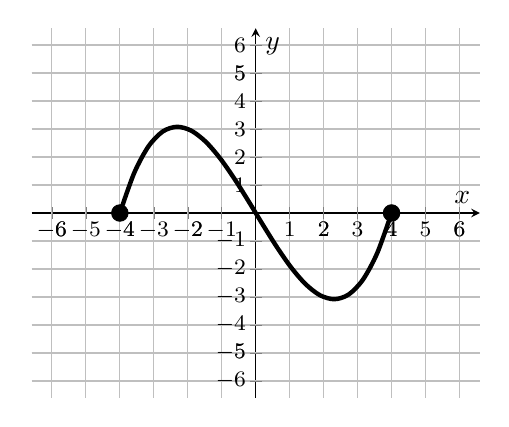
\begin{tikzpicture}
\begin{axis}[
   grid = major,
   extra x ticks={-6,-5,-4,-3,-2,-1,1,2,3,4,5,6},
   extra y ticks={-6,-5,-4,-3,-2,-1,1,2,3,4,5,6},
   %xminorgrids=true,
   width=.6\textwidth,
   %clip = true,
   %clip mode=individual,
   %restrict y to domain=-12:12,
   axis x line = middle,
   axis y line = middle,
        yticklabel style = {font=\footnotesize,xshift=0.5ex},
        xticklabel style = {font=\footnotesize,yshift=0.5ex},
   xlabel={$x$},
   %xlabel style={at=(current axis.right of origin)},
   ylabel={$y$},
   %ylabel style={at=(current axis.above origin)},
   %domain = -5:5,
   xmin = -6,
   xmax = 6,
   enlarge y limits={rel=0.05},
   enlarge x limits={rel=0.05},
   ymin = -6,
   ymax = 6,
 ]
% \addplot[smooth, ultra thick, domain = -5:-2,samples=2
% 	] { (-2*x)-4}
%  node[pos=.95](endofplotsquare){} ;
 \addplot[smooth, ultra thick, domain = -4:4,samples=20
	] { .125*x^3-2*x}
 node[pos=.95](endofplotsquare){} ;
%\node [right] at (endofplotsquare) {$f(x)$};%
        % \addplot[only marks,mark=*, mark options={scale=2, fill=white}, line width=0.3pt, mark size=1.5pt] coordinates{(-2,0) (5,0)};
         \addplot[only marks,mark=*, mark options={scale=2, fill=none}, line width=0.3pt, mark size=1.5pt] coordinates{(-4,0) (4,0)};
\end{axis}
\end{tikzpicture}
\begin{checkboxes}
    \choice The graph \underline{is} a function and \underline{does} have an inverse.
    \choice The graph is \underline{not} a function does \underline{not} have an inverse.
    \choice The graph is \underline{not} a function, but \underline{does} have an inverse.
    \choice The graph \underline{is} a function, but does \underline{not} have an inverse.

    \choice None of the above.
\end{checkboxes}

\question[3] Consider a polynomial
\[P(x) = ax^n\]
You know $n$ is a positive integer, but do not know $a$. If as $x\to-\infty$ $P(x)\to+\infty$ and as $x\to+\infty$ $P(x)\to-\infty$. What do you know about $a$ and $n$?
\begin{checkboxes}
    \choice $a$ is positive and $n$ is odd.
    \choice $a$ is negative and $n$ is odd.
        \choice $a$ is negative and $n$ is even.
    \choice $a$ is positive and $n$ is even.

    \choice None of the above.
\end{checkboxes}

\newpage
\question[4] Here is a graph of the parent function $f(x)= \sqrt{x}$.
%\todo{By Decree of Travis: We will punt this question and come back to it.}
        \begin{center}
            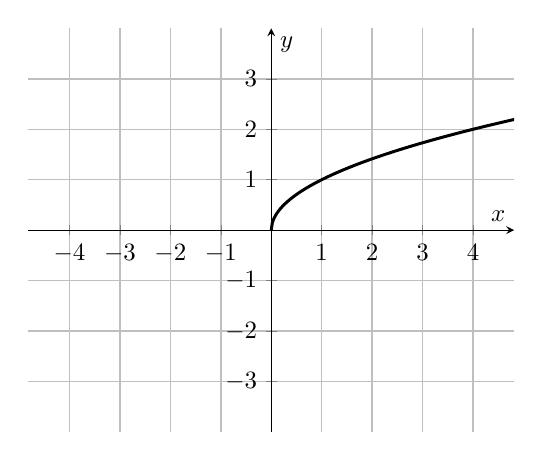
\begin{tikzpicture}[scale=0.9]
                          \begin{axis}[
                            domain=0:5,
                            samples=100,
                            xmin=-4, xmax=4,
                            ymin=-4, ymax=4,
                            axis equal,
                            axis lines=middle,
                            xlabel={$x$},
                            ylabel={$y$},
                            xtick={-4,-3,-2,-1,0,1,2,3,4},
                            ytick={-3,-2,-1,0,1,2,3},
                            grid=both,
                            minor grid style={dotted},
                            major grid style={semithick}
                          ]
                             \addplot[black, very thick, samples=250] {sqrt((x))};
                            \end{axis}
            \end{tikzpicture}
        \end{center}

Match each function child function below to its graph. Write the letter of the corresponding graphs in the boxes next to the functions below.

    \begin{multicols}{2}
        \begin{enumerate}
            \item[(A)] 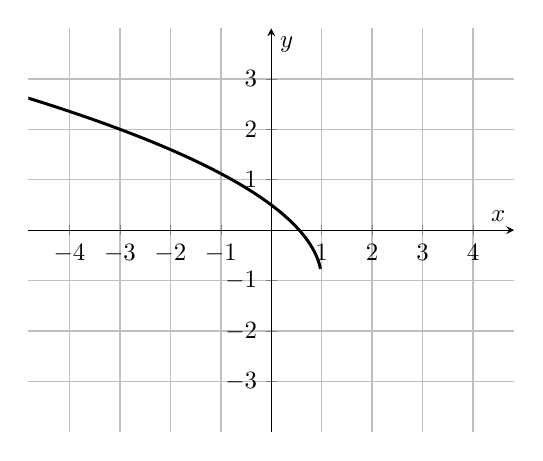
\begin{tikzpicture}[scale=0.9]
                      \begin{axis}[
                        domain=-5:1,
                        samples=100,
                        xmin=-4, xmax=4,
                        ymin=-4, ymax=4,
                        axis equal,
                        axis lines=middle,
                        xlabel={$x$},
                        ylabel={$y$},
                        xtick={-4,-3,-2,-1,0,1,2,3,4},
                        ytick={-3,-2,-1,0,1,2,3},
                        grid=both,
                        minor grid style={dotted},
                        major grid style={semithick}
                      ]
                         \addplot[black, very thick, samples=250] {1.5*sqrt(-x+1)-1};
                         %\node at (axis cs: 2,1.5) [anchor=north west] {$\mathbf{f(x)}$};
                        \end{axis}
                \end{tikzpicture}
                
            \item[(B)] 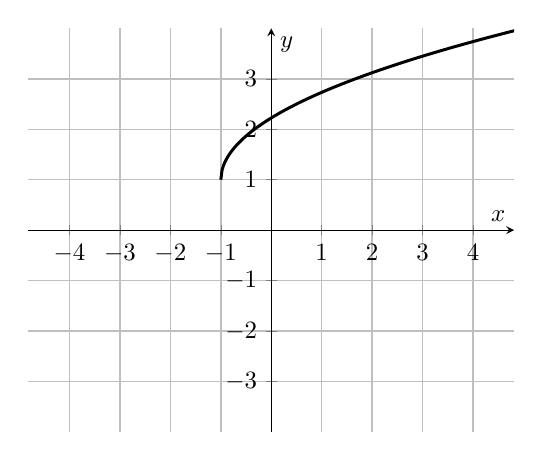
\begin{tikzpicture}[scale=0.9]
                      \begin{axis}[
                        domain=-1:5,
                        samples=100,
                        xmin=-4, xmax=4,
                        ymin=-4, ymax=4,
                        axis equal,
                        axis lines=middle,
                        xlabel={$x$},
                        ylabel={$y$},
                        xtick={-4,-3,-2,-1,0,1,2,3,4},
                        ytick={-3,-2,-1,0,1,2,3},
                        grid=both,
                        minor grid style={dotted},
                        major grid style={semithick}
                      ]
                         \addplot[black, very thick, samples=250] {sqrt((3/2)*(x+1))+1};
                         %\node at (axis cs: 2,1.5) [anchor=north west] {$\mathbf{f(x)}$};                 
                        \end{axis}
                \end{tikzpicture}
                
                
            \item[(C)] 
            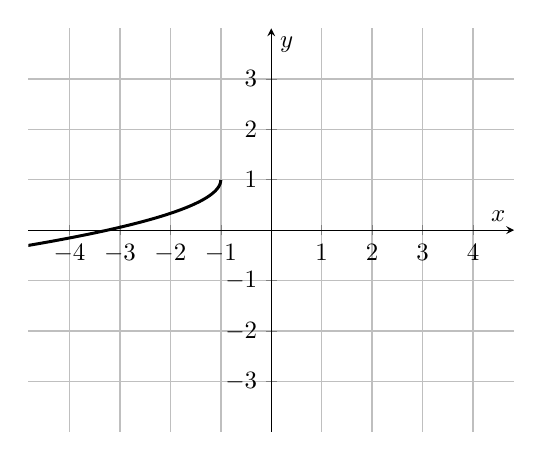
\begin{tikzpicture}[scale=0.9]
                      \begin{axis}[
                        domain=-5:-1,
                        samples=500,
                        xmin=-4, xmax=4,
                        ymin=-4, ymax=4,
                        axis equal,
                        axis lines=middle,
                        xlabel={$x$},
                        ylabel={$y$},
                        xtick={-4,-3,-2,-1,0,1,2,3,4},
                        ytick={-3,-2,-1,0,1,2,3},
                        grid=both,
                        minor grid style={dotted},
                        major grid style={semithick}
                      ]
                         \addplot[black, very thick, samples=500] {-(2/3)*sqrt(-x-1)+1};
                         %\node at (axis cs: 2,1.5) [anchor=north west] {$\mathbf{f(x)}$};                 
                        \end{axis}
                \end{tikzpicture}
                
            \item[(D)] 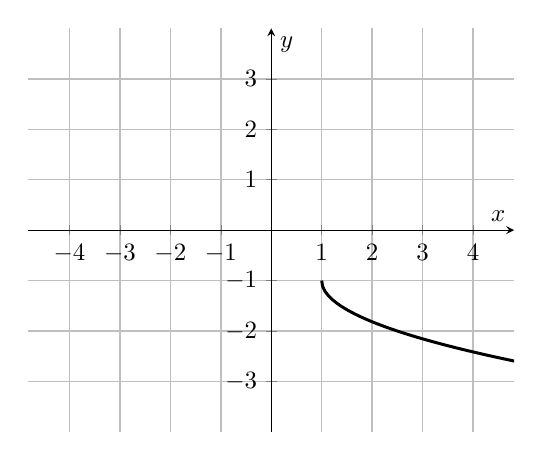
\begin{tikzpicture}[scale=0.9]
                      \begin{axis}[
                        domain=1:5,
                        samples=100,
                        xmin=-4, xmax=4,
                        ymin=-4, ymax=4,
                        axis equal,
                        axis lines=middle,
                        xlabel={$x$},
                        ylabel={$y$},
                        xtick={-4,-3,-2,-1,0,1,2,3,4},
                        ytick={-3,-2,-1,0,1,2,3},
                        grid=both,
                        minor grid style={dotted},
                        major grid style={semithick}
                      ]
                         \addplot[black, very thick, samples=250] {-1*sqrt((2/3)*(x-1))-1};
                         %\node at (axis cs: 2,1.5) [anchor=north west] {$\mathbf{f(x)}$};
                        \end{axis}
                \end{tikzpicture}
        \end{enumerate}
    \end{multicols}

   
    \begin{multicols}{2}
        $\boxed{\phantom{\dfrac{aaa}{b}}}$ =$\displaystyle -\frac{2}{3}\sqrt{-x-1}+1$\vspace{0.5cm}
        
        $\boxed{\phantom{\dfrac{aaa}{b}}}$ = $\displaystyle -\sqrt{\frac{2}{3}(x-1)}-1$ \vspace{0.5cm}
           
        $\boxed{\phantom{\dfrac{aaa}{b}}}$ = $\displaystyle \sqrt{\frac{3}{2}(x+1)}+1$ \vspace{0.5cm}
        
        $\boxed{\phantom{\dfrac{aaa}{b}}}$ = $\displaystyle \frac{3}{2}\sqrt{-x+1}-1$ \vspace{0.5cm}
    \end{multicols}



\newpage

 \question[3] Select the graph of $f(x)=x^2(x-2)^2$.
    
    \begin{multicols}{2}
    	
    	
    	\begin{choices}
    		\choice \chooseone\vspace{-.7cm}
    		
    		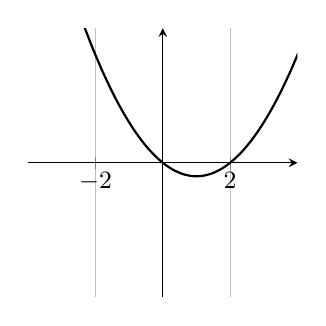
\begin{tikzpicture}%[domain=-4:4]
	\begin{axis}[
		grid=major,
		axis x line = middle,
		axis y line = middle,
		%yticklabel style = {font=\tiny,xshift=0.5ex},
		xticklabel style = {font=\small,yshift=0.5ex},
		%scale only axis=true,
		width=5 cm,
		height=5 cm,
		xtick={-2,0,2},%{-2,-1,0,1,2},
		ytick=false,%{-2,-1,0,1,2,3,4},
		xmin=-4,
		xmax=4,
		ymin=-10,
		ymax=10,
		]
		%\draw[very thin,color=gray] (-2.9,-2.1) grid (2.9,2.9);
		\addplot[smooth, thick, domain = -5:5,samples=35] { x*(x-2)};
		%\addplot[smooth, thick, domain = 0:3,samples=35] { -x};
	\end{axis}
\end{tikzpicture}
     
    		\choice \chooseone\vspace{-.7cm}
    		
    		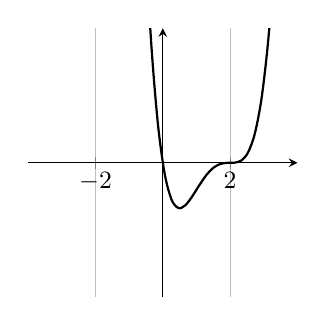
\begin{tikzpicture}%[domain=-4:4]
    			\begin{axis}[
    				grid=major,
    				axis x line = middle,
    				axis y line = middle,
    				%yticklabel style = {font=\tiny,xshift=0.5ex},
    				xticklabel style = {font=\small,yshift=0.5ex},
    				%scale only axis=true,
    				width=5 cm,
    				height=5 cm,
    				xtick={-2,0,2},%{-2,-1,0,1,2},
    				ytick=false,%{-2,-1,0,1,2,3,4},
    				xmin=-4,
    				xmax=4,
    				ymin=-5,
    				ymax=5,
    				]
    				%\draw[very thin,color=gray] (-2.9,-2.1) grid (2.9,2.9);
    				\addplot[smooth, thick, domain = -2:5,samples=35] { x*(x-2)^3};
    				%\addplot[smooth, thick, domain = 0:3,samples=35] { -x};
    			\end{axis}
    		\end{tikzpicture}
    		\\
    		\choice \chooseone\vspace{-.7cm}
    		
    		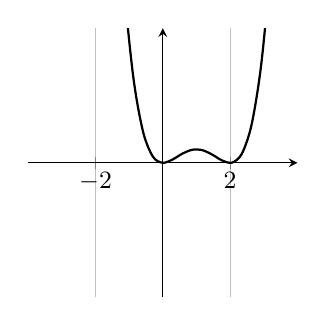
\begin{tikzpicture}%[domain=-4:4]
	\begin{axis}[
		grid=major,
		axis x line = middle,
		axis y line = middle,
		%yticklabel style = {font=\tiny,xshift=0.5ex},
		xticklabel style = {font=\small,yshift=0.5ex},
		%scale only axis=true,
		width=5 cm,
		height=5 cm,
		xtick={-2,0,2},%{-2,-1,0,1,2},
		ytick=false,%{-2,-1,0,1,2,3,4},
		xmin=-4,
		xmax=4,
		ymin=-10,
		ymax=10,
		]
		%\draw[very thin,color=gray] (-2.9,-2.1) grid (2.9,2.9);
		\addplot[smooth, thick, domain = -5:5,samples=35] { x^2*(x-2)^2};
		%\addplot[smooth, thick, domain = 0:3,samples=35] { -x};
	\end{axis}
\end{tikzpicture}
    		\choice \chooseone\vspace{-.7cm}
    		
    		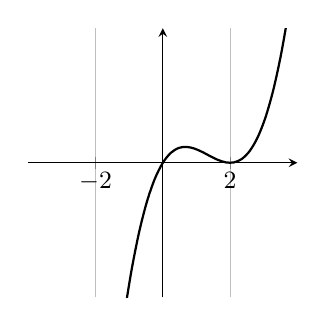
\begin{tikzpicture}%[domain=-4:4]
	\begin{axis}[
		grid=major,
		axis x line = middle,
		axis y line = middle,
		%yticklabel style = {font=\tiny,xshift=0.5ex},
		xticklabel style = {font=\small,yshift=0.5ex},
		%scale only axis=true,
		width=5 cm,
		height=5 cm,
		xtick={-2,0,2},%{-2,-1,0,1,2},
		ytick=false,%{-2,-1,0,1,2,3,4},
		xmin=-4,
		xmax=4,
		ymin=-10,
		ymax=10,
		]
		%\draw[very thin,color=gray] (-2.9,-2.1) grid (2.9,2.9);
		\addplot[smooth, thick, domain = -4:4,samples=35] { x*(x-2)^2};
		%\addplot[smooth, thick, domain = 0:3,samples=35] { -x};
	\end{axis}
\end{tikzpicture}

      \choice \chooseone None of the above.
    	\end{choices}
    \end{multicols}
    \newpage
\hspace{-.5in}Free answer section. Work must be shown to get credit for any answer. Partial credit may be given even for incorrect final answers, so show your work.

\question %alejandro
Every $3$ years, an average family in the US generates $10$ tons of trash. Your family created $95$ tons of waste before you were born. Let $x$ represent years after your birth. \vspace{.2in}
\begin{parts}
\part[3] Find a linear function $w=f(x)$ that determines the total amount of waste created by an average family $w$ as a function of time $x$. \vspace{1.5in}
\part[3] Find $f(21)$ and explain what it tells you in this situation. \vspace{1.5in}
\part[3] Find $x=f^{-1}(w)$ for value of $w$. \vspace{2in}
\part[3] Find $f^{-1}(205)$ and explain what it tells you in this situation.     
\end{parts}
%Data can be tweaked for makeup exams, making sure to get integer slope for the rate of children arrested and nice fractions for f^-1. E.g. f(0)=400 000, f(x)=200 000 + 60 000 x child arrests at the border, and ask for the year=f^-1(2 000 000) 


\newpage
\question[10]
%Taeyoung's problem on sec 3.3
Perform the polynomial long division, then identify the quotient and the remainder.
    \begin{equation*}
        \left(x^4+3 x^3+5x^2+2x+1\right) \div\left(x^2+1\right)
    \end{equation*}
    



\newpage
% Penny: section 3.1, quadratics
\question Suppose a ball is thrown directly upward, and its height (in feet) after $t$ seconds is given by 
\[
y(t) = - 16 t^2 + 16t + a\,, \quad (\mathrm{ft})
\]
with $a$ to be determined.

\begin{parts}
\part[2] If at time $t=0$, the ball is thrown at height $10 \mathrm{ft}$, what is the value of $a$?
% 1 pt: if correct a=10
\vfill

\part[6] Write the function $y(t)$ in vertex form by completing the square.
% 1pt: correct h
% 1pt: correct coefficient a
% 1pt: correct completing the square b^2 term
% 1pt: correct k
\vfill\vfill\vfill

\part[3] When does the ball reach its maximum height? What is the maximum height? Please include units for both answers.
% 1pt: t=1/2
% 1pt: y=14
% 1pt: correct unitsx2
\vfill
        \begin{multicols}{2}
            $
                \mbox{Max Height: } \Scale[1.1]{\boxed{ \phantom{\frac{a}{b}} \hspace{3cm} }}
            $
            \\
            $
                \mbox{Time: } \Scale[1.1]{\boxed{ \phantom{\frac{a}{b}} \hspace{3cm} }}
            $
            \end{multicols}


\end{parts}
\newpage
\question %Building Polynomials

    \begin{parts}
    \part[6] Find the polynomial $h(x)$ of  least possible degree with \underline{integer coefficients} %and a repeated root $1 + 2i$ with multiplicity $2$ such that $f(1) = 50$ and $f(3) = 0$. %We have said the complex roots aren't on this exam
    that has a repeated root of $-3$ with multiplicity 2 and a root of 
    $\sqrt{5}$ 
    such that $h(0)=90$.
    
    (You may leave your answer as a product of linear factors.)
    
    %Grading Notes: the extra root at -sqrt(2) worth at most 1 point
    
    \vfill\vfill\vfill
    
    %\vfill
    \part[4] What is the leading term of the polynomial and what is the degree of the polynomial?
    %Determine all the roots of $f(x)$ and their corresponding multiplicity.
    %\todo{Could we change this part to asking: what is the degree of $f$, what is the leading term, and what is the constant term?}
    \vspace{1cm}
    
        \begin{multicols}{2}
            $
                \mbox{Leading term: } \Scale[1.1]{\boxed{ \phantom{\frac{a}{b}} \hspace{3cm} }}
            $
            \\
            $
                \mbox{Degree: } \Scale[1.1]{\boxed{ \phantom{\frac{a}{b}} \hspace{3cm} }}
            $
            \end{multicols}
    \end{parts}
    

    
% \end{parts}



\newpage
\newpage
\question Compute the following. %Anuk
\begin{parts}
\part[3] Let $f(x) = \dfrac{1}{2-x}$ and $g(x) = \sqrt{x+12}.$ Let $h(x) = \dfrac{f(x)}{g(x)}.$ Compute $h(4).$ \vfill%\vspace{1.5in}
\part[4] Let $p(x) = \sqrt{-x + 6}$ and $q(x) = \sqrt{x-1}$. Let $r(x) = p\cdot q(x)$. Find the domain of $r(x)$.% and compute $r(3).$ 
\vfill\vfill%\vspace{2.5in}
\part[4] Let $a(x) = \dfrac{1}{5-x}$ and $b(x) = x^2+1$. Compute $a \circ b(x)$ and find its domain.\vfill\vfill
\end{parts}
\newpage

%\question  %Ari
%\begin{parts}
    \question[8] Let $f(x)=\dfrac{3}{x+4}$. Find $f^{-1}(x)$, and find the domain of $f(x)$.
    \vspace{3.5in}
    \newpage
        \question Let $g(x)=\sqrt{x+4}+1$. The graph is shown below.
        
               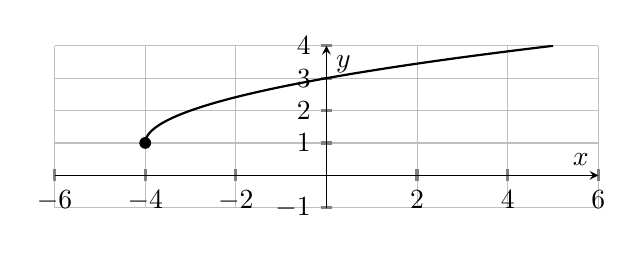
\begin{tikzpicture}
\begin{axis}[
  width= .7\textwidth,
  height= .3\textwidth,
  axis lines=middle,
  grid=major,
  xmin=-6,
  xmax=6,
  ymin=-1,
  ymax=4,
  xlabel=$x$,
  ylabel=$y$,
  xtick={-12,-10,...,10},
  ytick={-2,-1,...,6},
  tick style={very thick},
  % legend style={
  % at={(rel axis cs:0,1)},
  % anchor=north west,draw=none,inner sep=0pt,fill=gray!10}
]
\addplot[smooth, thick, domain = -3:5,samples=30] { sqrt(x+4)+1};
\addplot[smooth, thick, domain = -4:-3,samples=30] { sqrt(x+4)+1};
\node at (axis cs:-4,1) [circle,fill=black,inner sep=1.5pt] {};
%\addplot[smooth, thick, domain = -3.85:-3,samples=30] { (2*x-5)/(x+4)};
%\addplot[smooth, thick, domain = -3:10,samples=30] { (2*x-5)/(x+4)};
%\addplot[dashed, domain =-12:8, samples = 2]{2};
%\draw[dashed](axis cs:-4, -14) -- (axis cs:-4, 20);
\end{axis}
\end{tikzpicture}
    \begin{parts}
        \part[2] What is the domain and range of $g(x)$? (Write in interval notation.)
        \begin{multicols}{2}
            $
                \mbox{Domain: } \Scale[1.1]{\boxed{ \phantom{\frac{a}{b}} \hspace{3cm} }}
            $
            \\
            $
                \mbox{Range: } \Scale[1.1]{\boxed{ \phantom{\frac{a}{b}} \hspace{3cm} }}
            $
            \end{multicols}
%\vfill
        \part[6] What is $g^{-1}(x)$?
\vfill
$
                g^{-1}(x) = \Scale[1.2]{\boxed{ \phantom{\dfrac{a}{b}} \hspace{5cm} }}
            $
        \part[2] What are the domain and range of $g^{-1}(x)$? %(Write in interval notation.)
        \begin{multicols}{2}
            $
                \mbox{Domain: } \Scale[1.1]{\boxed{ \phantom{\frac{a}{b}} \hspace{3cm} }}
            $
            \\
            $
                \mbox{Range: } \Scale[1.1]{\boxed{ \phantom{\frac{a}{b}} \hspace{3cm} }}
            $
            \end{multicols}


    \end{parts}

% \newpage

%\end{parts}

\newpage
\question %\textbf{[Section 3.4\&3.5]} 
    Let $f(x)= 3 x^3 - 13 x^2 - 11 x + 5$. %Roots x= -1, 5, 1/3
    %
    %or 
    %$f(x)=
    \begin{parts}
    \part[2] List all possible rational roots of $f(x)$ according to the rational root theorem.
    \vfill
    
    \part[8] We know that $f(x)$ has a root at $x=5$. Use this fact to find all the roots of $f(x)$.
    
    \vfill\vfill\vfill
    
    \part[2] Write $f(x)$ as a product of linear factors.
    \vspace{1.5cm}
    
    $
                \mbox{$f(x)=$ } \Scale[1.5]{\boxed{ \phantom{\frac{a}{b}} \hspace{8cm} }}
            $
    \end{parts}

\newpage
SCRATCH PAPER




\newpage

SCRATCH PAPER










\end{questions}





\end{document}
